% Write about tensorflow 
    %   - short background on tensorflow
    %   - ways of training/ new architecture (code or config), new model existing layout , transfer learning
    %   - setup for training (cpu, gpu, cuda, cudnn)
    %   - short background on cuda and cudnn
    %   - training a model
    %   - analysis of model
\begin{document}
TensorFlow™ is an open source software library for high performance numerical computation. Its flexible architecture allows easy deployment
of computation across a variety of platforms (CPUs, GPUs, TPUs), and from desktops to clusters of servers to mobile and edge devices.
Originally developed by researchers and engineers from the Google Brain team within Google’s AI organization, it comes with strong support
for machine learning and deep learning and the flexible numerical computation core is used across many other scientific
domains.\cite{tensorflow}

\section{Writing Object Detection Models with Tensorflow}\label{train-with-tensorflow}
Tensorflow is a full fledged machine learning framework which support the programming languages C++, Python. It is multi purpose framework
which can be used for training Neural Networks for Image Recognition, Object Detection or other purposes. Furthermore tensorflow uses
Keras which is a high level API for building and training deep learning models. For Object Detection for which I am using Tensorflow in this
report, you are able to write a Object Detection Neural Network in multiple ways.
\begin{itemize}
    \item Do it Yourself \\ \\
        You are able to write your object detection logic from scratch, starting at how features are being extracted processed and
        evaluated to how layers of your neural networks are connected, sequenced, communicate and how the object localization and object
        classification is being used and implemented.
    \item Just write the Model \\ \\
        Tensorflows object detection model which they provide at \url{https://github.com/tensorflow/models} is a simple yet effective way of
        training Object Detection Neural Netowrks. You are able to compose new ideas for models with simple '.config' files without going
        too deep into the code and logic of tensorflow. These config files contain the setup of the neural network model. For instance in
        which sequence the layers are going to be, what the IoU value has to be for a bounding box to be valid and which features have to
        bextracted by the tensorflow api. See appendix\ref{tfconfig} for a full '.config' file used for training.
\end{itemize}

\section{Training Models with Tensorflow}\label{models-with-tensorflow}
As there are multiple ways of setting up your neural network there are also a couple of ways training it. It start with the choice of your
dataset, it can bias orientated meaning that it will recognize one type of image very good but fail on others, in machine learning terms it
overfitts. Or it can be 
\begin{itemize}
    \item Train from Scratch \\ \\
        Which ever way you are training your model, starting from scratch without a basis will require: \\
        {- alot of resources (images, ground truth data)} \\
        {- alot of training time} \\
    \item Train by transfer Learning \\ \\
        When you are doing transfer learning, you are taking an already trained model and build ontop of it with your own image set.\\
        This results in: \\
        {- far fewer images need} \\
        {- less training time (comparing days and weeks to hours and minutes)} \\
\end{itemize}
Training is pretty straight forward when using the setup from tensorflow as mentioned in\ref{train-with-tensorflow} "Just write the Model".
For this you have to install Tensorflow and all the required dependencies. They can be found here:
\url{https://www.tensorflow.org/install/pip}. Futhermore some custom scripts were written to enable convertig txt files to .csv files to
enable the generation of .record files and to merge entries of multiple files with the same naming (there were multiple files with the same
name and content but labeled differently for each category). Lastly environmental variables, proto
files and '.record' files had to be setup, compiled for tensorflow.
\begin{center}
    \begin{tabular}{|c|c|c|c|c|}
        \hline
        Model & Speed(ms) &  mAP[{\textasciicircum}1] \\ \hline
        faster-rcnn-inception-v2-cooc & 58 & 28 \\ \hline
        ssd-mobilenet-v2-coco & 32 & 22 \\ \hline
    \end{tabular}
\end{center}
\section{Training results}
After setting up the environment my first attempt was getting the data myself, labeling them with the Open Source software
\href{https://github.com/tzutalin/labelImg}{LabelImg} and training a new Model through a tensorflow config. This was a tedious effort and
resulted in a bad model which detected images pretty well as long as they were from the train set or similiar but failed on real world data.
This was done with various combinations of data quantities which was not enough at all for this, IoU, variable and feature tweaks provided
through Tensorflow without much difference in its performance. To note is that these were my first attempts training models with tensorflow
and I did not understand the whole procedure too well, meaning I didn't consult tensorboard which is User Interface from Tensorflow to view
the results of my Data and Model. \\ 
After this I switched to transfer learning which takes the weights and knowledge of a already
\href{https://github.com/tensorflow/models/blob/master/research/object_detection/g3doc/detection_model_zoo.md}{existing models} from
tensorflow and applies it to a different one with related problems. \\ 
Firstly I downloaded images and bounding box data through the api of ms coco which is a dataset providing more then 2.5 million labele
instances in 328k images.\cite{mscoco} There are other datasets such as Pascal VOC and ImageNet but none of them provided a easy way to
download data similar to MSCOCO. For the following models I downloaded 9 Classes with 1k images and labels each to test, vary and experiment
with the amount of data provided to training my model. \\
Secondly I donwloaded two models from tensorflow, one was the faster-rcnn-inception-v2-coco and the ssd-mobilnet-v2-coco trained with the
dataset from MSCOCO. These are 2 models where the first one is implemented with the Faster-RCNN and the later with SSD algorithm. \\
When transfer learning I noticed that 200 images for each category was more then enough to get decent results, the results degraded compared
to the original Tensorflow models I used for transfer learning but it was still better then the intial attempts of training. The following
graphs are smoothed by a factor of 0.6. \\ \\
\begin{figure}[hbt!]
    \begin{center}
        \caption{mAP}
        \subfigure[mAP per Stage]{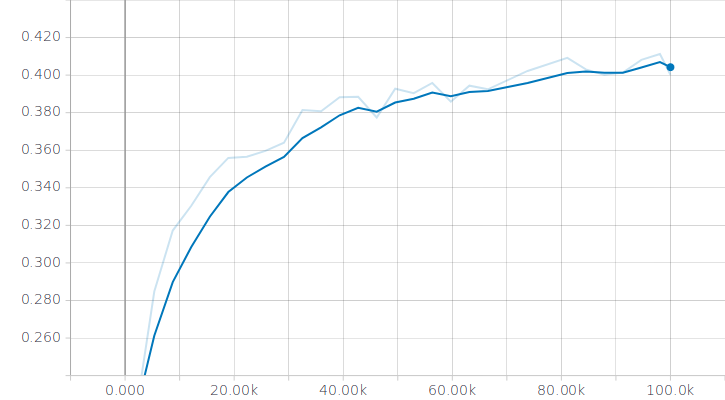
\includegraphics[scale=0.3]{images/tensorflow/frcnn-map.png}}
        \subfigure[mAP @0.5 IoU]{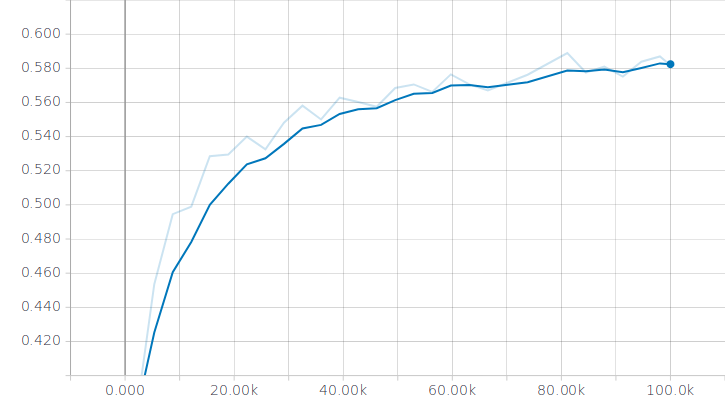
\includegraphics[scale=0.3]{images/tensorflow/frcnn-map@0-50iou.png}}
        \subfigure[mAP @0.75 IoU]{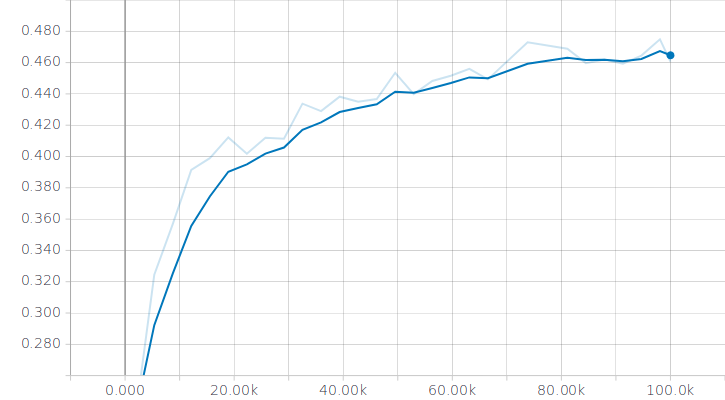
\includegraphics[scale=0.3]{images/tensorflow/frcnn-map@0-75iou.png}}
    \end{center}
\end{figure}
\newpage
\noindent
Even though the mAP is increasing over the duration of the training session you can see that it is not really increasing in performance but
overfitting through the following grpahs:
\begin{figure}[hbt!]
    \begin{center}
        \caption{Loss of Models}
        \subfigure[Box Classifier Loss]{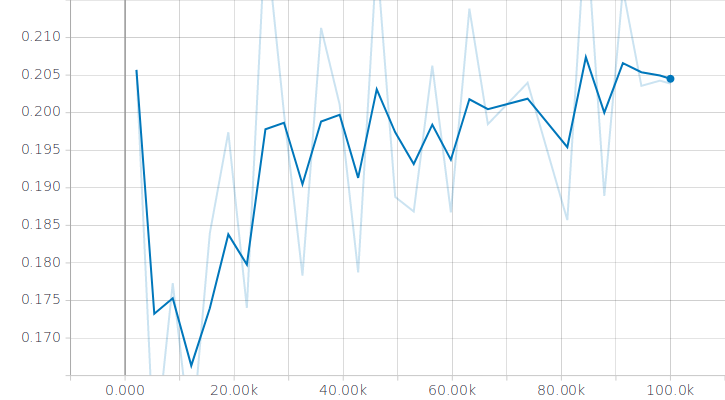
\includegraphics[scale=0.3]{images/tensorflow/frcnn-classification_loss.png}}
        \subfigure[Box Classifier Localization Loss]{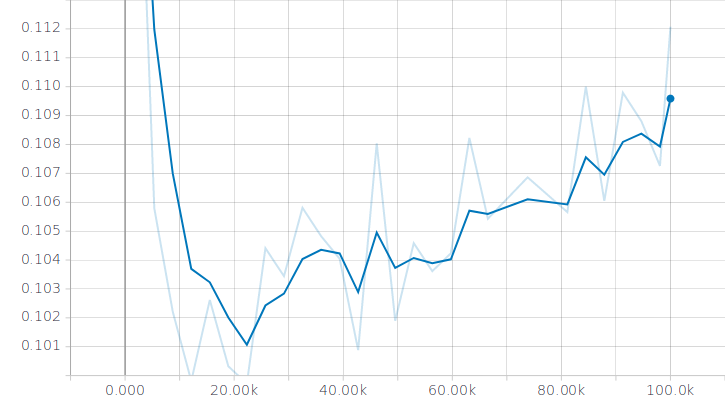
\includegraphics[scale=0.3]{images/tensorflow/frcnn-box_localization_loss.png}}
        \subfigure[RPN Localization Loss]{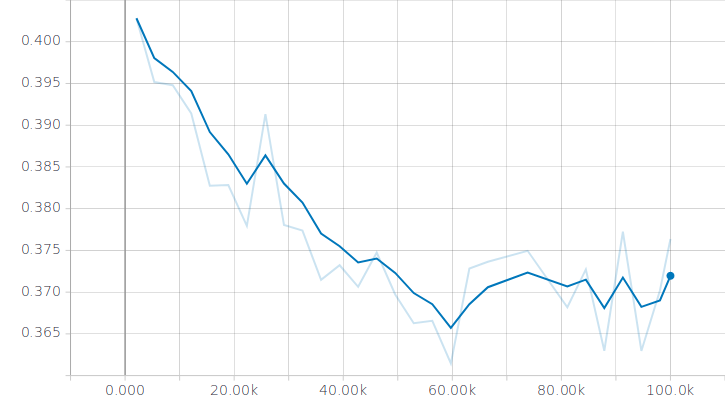
\includegraphics[scale=0.3]{images/tensorflow/frcnn-rpn_localization_loss.png}}
        \subfigure[RPN Objectness Loss]{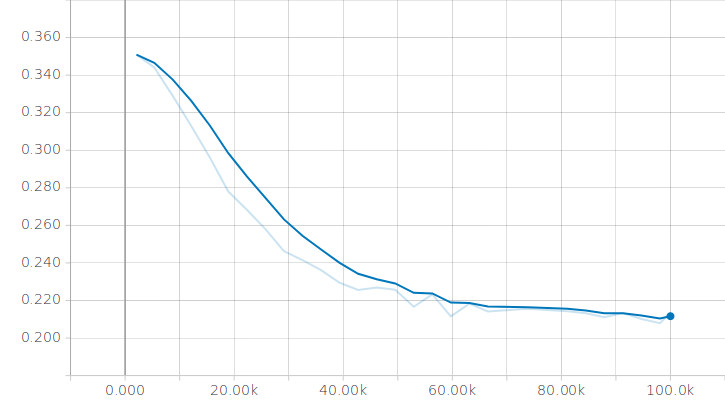
\includegraphics[scale=0.3]{images/tensorflow/frcnn-rpn_objectness_loss.png}}
        \subfigure[Total Loss]{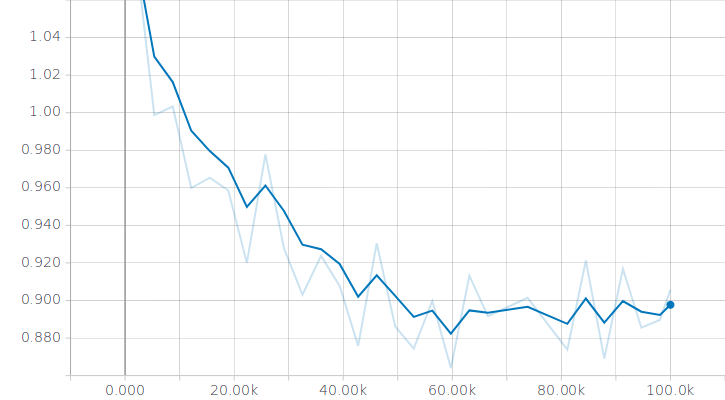
\includegraphics[scale=0.3]{images/tensorflow/frcnn-total_loss.png}}
    \end{center}
\end{figure}
\end{document}
